\documentclass[a4paper]{article}
\usepackage[a4paper, top=1in, left=1.2in, right=1.2in, bottom=1in, footskip=0.25in]{geometry}
\usepackage[absolute]{textpos}
\usepackage{subfigure}
\usepackage{float}
\usepackage{hyperref}
\usepackage{graphicx}
\usepackage{blindtext}
\usepackage{array}
\usepackage{tabularx}
\usepackage{pgfplots}
\usepackage{pgf-umlcd}
\usepackage{tikz}
\usepackage[T1]{fontenc}
\usepackage{listings}
\pgfplotsset{width=10cm,compat=1.9}
\graphicspath{ {./images/} }
\bibliographystyle{ieeetr}

% enum style and environment from
% https://github.com/jcb/these-jcb/blob/master/custom_pgf-umlcd.sty
% Author: Jean-Christophe Bach
\tikzstyle{umlcd style enum}=[rectangle split, rectangle split parts=2, 
every text node part/.style={text centered},
draw, minimum height=2em, umlcolor, minimum width=2cm, text width=4cm,
minimum height=1cm, node distance=2cm]
\newenvironment{enum}[3][]%
{
\begin{classAndInterfaceCommon}{#1}{#2}{#3}
}%
{\node[umlcd style enum, anchor=north] (\umlcdClassName) at (\umlcdClassPos)
    {$<<$enumeration$>>$ \\ \textbf{\umlcdClassName}
\nodepart{second}
\umlcdClassAttributes
};
\end{classAndInterfaceCommon}
}

\title{
	Currying the web: A custom Java REST framework - built on functional paradigms
	- compared to Spring Boot: Performance, Developer Guidance and Ease of Use
}
\author{Nico Lerchl\\2110257236\\[0.5cm]{\small Advisor: Dipl.-Ing. (FH) Bernhard Wallisch}}

\begin{document}

\begin{textblock}{15}(0.5, 0.5)
	\noindent\Large BACHELOR PAPER\\
	\large Thesis submitted in fulfillment of the requirements for the degree of Bachelor
	of Science in Engineering at the University of Applied Sciences Technikum Wien
	- Degree Program Computer Science
\end{textblock}

\maketitle

\newpage

\section*{Declaration}
“As author and creator of this work to hand, I confirm with my signature knowledge of the relevant
copyright regulations governed by higher education acts (see Urheberrechtsgesetz / Austrian
copyright law as amended as well as the Statute on Studies Act Provisions / Examination
Regulations of the UAS Technikum Wien as amended).\newline

\noindent I hereby declare that I completed the present work independently and that any ideas, whether
written by others or by myself, have been fully sourced and referenced. I am aware of any con-
sequences I may face on the part of the degree program director if there should be evidence of
missing autonomy and independence or evidence of any intent to fraudulently achieve a pass
mark for this work (see Statute on Studies Act Provisions / Examination Regulations of the UAS
Technikum Wien as amended).\newline

\noindent I further declare that up to this date I have not published the work to hand nor have I presented
it to another examination board in the same or similar form. I affirm that the version submitted
matches the version in the upload tool.“


\newpage
\section*{Kurzfassung}
\blindtext
\newline

\noindent Keywords: REST, Java, Funktionale Programmierung, Spring Boot


\newpage
\section*{Abstract}
\blindtext
\newline

\noindent Keywords: REST, Java, functional programming, Spring Boot

\newpage
\section*{Acknowledgements}
\blindtext

\newpage

\tableofcontents

\newpage

\section{Introduction}

Web development is a huge part of the software industry. Most of the time, the
server part of a web application is built using the MVC pattern and object
oriented programming \cite{damir2021architecture}. Functional programming is not
used as much in web development, in the last few years however, functional
programming has been gaining a lot of popularity with languages such as Haskell,
Scala and Clojure but also with functional concepts being added to object
oriented languages like Java and C\# \cite{klint2022functional}.\newline

\noindent Combining functional programming with web development using more
widely used languages e.g. Java is a scarcely researched topic which this thesis
aims to explore and shine some light on. The goal is to build a REST framework
using functional paradigms and compare it to Spring Boot in terms of
performance, developer guidance and ease of use.

\section{Literature review}
\subsection{REST}

Representational State Transfer (REST) is the state-of-the-art way to build the
server part of a client-server-architecture and it is most likely only going to
get bigger in the industry \cite{halili2018web}. It was first described by Roy
Fielding in his doctoral dissertation in 2000. REST is based on the following
properties \cite{fielding2000architectural}:

\begin{itemize}
	\item Client-server - The client and the server are separated and can be
	      developed independently.
	\item Stateless - The server does not store any client state. Every request
	      contains all the information the server needs to process it.
	\item Cache - Responses can be cached to improve performance.
	\item Uniform Interface - The interface between the client and the server is
	      uniform and simple.
\end{itemize}

\subsection{Functional programming}
\subsubsection{General}

Functional programming - unlike procedural or object oriented programming - is
not based on the Turing machine, but rather on lambda calculus. Lambda calculus,
developed by Alonzo Church in the 1930s, is a mathematical system later proven -
by Turing himself - to be equivalent to the Turing machine
\cite{turing1937computability}.\newline

\noindent The base principles of functional programming are
\cite{hughes1989functional}:
\begin{itemize}
	\item Immutability - Variables are not changed after they are assigned a
	      value.
	\item Pure functions - Functions do not have side effects and always return
	      the same output for the same input.
	\item Higher order functions - Functions can be passed as arguments to other
	      functions.
	\item Referential transparency - A function call can be replaced by its
	      return value without changing the program's behavior.
\end{itemize}

\noindent A big part of functional programmings is the concept of monads which
have their roots in category theory. They allow for encapsulating side effects
in a pure way. For a container to be a monad it has to abide by the laws of left
identity, right identity and associativity. \cite{wadler1992essence}

\subsubsection{Web development}

Yesod is a web framework for the before mentioned functional programming
language Haskell. It allows developers to build entire websites using templates
and widgets or RESTful web services. Additionally, Yesod offers the ability to
persist data using Haskell's type system into PostgreSQL, SQLite, MySQL, and
MongoDB. \cite{snoyman2015developing}

\subsubsection{In Java}

The introduction of lambda expressions in Java 8 brought functional programming
to the Java ecosystem. Where before developers had to use anonymous classes to
pass functions as arguments, they can now use lambda expressions. This also
shifts the view point of passing an object that carries functionality to passing
behavior itself. The concept behind these lambda expressions in Java is called
functional interfaces. Functional interfaces are interfaces that have exactly
one abstract method. They can be annotated with \verb|@FunctionalInterface|.
\newline

\noindent Also new to Java 8 is the Streams API. It hides away the iteration
over collections by offering many higher order functions. Additionally, streams
are only evaluated when a terminal operation, such as collecting, counting or
averaging is called, implementing the - before mentioned - functional
programming principle of lazy evaluation. \cite{warburton2014java}

Java 8 also saw the introduction of the \verb|Optional|-class. It is a container
that may or may not contain a non-null value. TODO

\subsection{Spring Boot}

Spring Boot is a framework for building stand-alone web applications and RESTful
web services in Java. Unlike Spring Framework there is zero requirement for XML
configuration. It can be deployed using an internal web server or going the
classic route of deploying a war file onto an external web server.
\cite{webb2013spring}

\section{Curryful}
Curryful tries to combine Java's simplicity with functional paradigms to build
better performant and unwanted behavior diminishing REST APIs, whilst offering
a great developer experience through easy use. As of now, when developing a REST
API using Curryful, one will require two dependencies: Curryful-commons and
curryful-rest. Having a dependency just for common functional programming tools
in Java allows for building any kind of application using functional paradigms
or enriching existing REST frameworks with functional utilities. Curryful is
hosted under a GitHub organization and can be found at
\url{https://github.com/Curryful}.

\subsection{Curryful-commons}
Curryful-commons offers a basis to writing functional Java code. It provides a
common abstract class for Monads and implementations for the Maybe and Try
monads. Since Java contains the before mentioned monadic Optional class, which
shares striking resemblance to the Maybe monad, the Maybe monad offers a
function to create a Maybe from an Optional. The Try monad allows for elegantly
handing exceptions in a functional way instead of throwing and catching them.

Though Java is always pass-by-value, anything but primitive types essentially
behave like pass-by-reference as object's references are passed by value.
\cite{hott2024java} This allows for objects to be mutated, without the caller
knowing, causing unwanted behavior and it also goes against the functional
principle of purity. To avoid this, curryful-commons offers mutable and
immutable variants of Java's \verb|ArrayList| and \verb|HashMap| where the
mutable collections inherit from the immutable ones. This way, the mutable ones
can be passed in place of their immutable counterparts, making it impossible for
the called function to mutate the parameters. This concept of "immutability
downcasts" is also referenced in "Javari: Adding Reference Immutability to Java"
\cite{tschantz2005javari} by Matthew S. Tschantz and Michael D. Ernst from the
University of Cambridge.

\begin{figure}[H]
	\begin{center}
		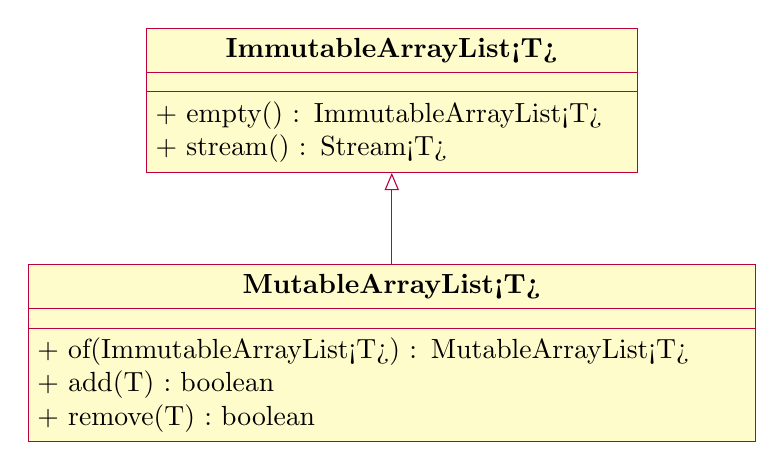
\begin{tikzpicture}
			\begin{class}[text width=6cm]{ImmutableArrayList<T>}{0,0}
				\operation{+ empty() : ImmutableArrayList<T>}
				\operation{+ stream() : Stream<T>}
			\end{class}

			\begin{class}[text width=9cm]{MutableArrayList<T>}{0,-3}
				\inherit{ImmutableArrayList<T>}
				\operation{+ of(ImmutableArrayList<T>) : MutableArrayList<T>}
				\operation{+ add(T) : boolean}
				\operation{+ remove(T) : boolean}
			\end{class}
		\end{tikzpicture}
	\end{center}
	\caption{(Incomplete - for clarity) class diagrams of ImmutableArrayList and
			MutableArrayList and their relationship}
\end{figure}

\noindent Additionally, curryful-commons provides a higher order function
Y-combinator to allow for recursion when using lambda expressions. This is
necessary because Java does not allow referencing a lambda expression before it
has been fully defined, e.g. from within itself.

\begin{center}
	\begin{lstlisting}[language=Java, caption=Example of using the Y-combinator,
			captionpos=b, ]
		Y(readHttp).apply(ImmutableArrayList.empty());
	\end{lstlisting}
\end{center}

\subsection{Curryful-rest}
In curryful-rest, everywhere possible, lambda expressions are used to define
functionality. This is done in a way where each lambda expression only takes one
input. This allows for currying whenever desired.

\subsubsection{HTTP}
Curryful-rest implements its own HTTP handling to build functionally from the
ground up. The \verb|HTTP|-Class offers methods to parse incoming requests and
serialize outgoing responses. All fetching of information from the request such
as method, path, headers, etc. is done using regular expressions. As visible in
figure \ref{figure:http-context-classes} and \ref{figure:http-response-classes},
Headers, path and query parameters are stored in immutable collections to
mitigate unwanted behavior. All other types used do not allow for mutation as
their fields are \verb|final| and no mutating methods are provided.

\begin{figure}[H]
	\begin{center}
		\begin{tikzpicture}
			\begin{class}[text width=10cm]{HttpContext}{0,0}
				\attribute{- actualUri : String}
				\attribute{- formalUri : String}
				\attribute{- pathParameters : ImmutableMaybeHashMap<String, String>}
				\attribute{- queryParamters : ImmutableMaybeHashMap<String, String>}
				\attribute{- headers : ImmutableMaybeHashMap<String, String>}
				\attribute{- address : InetAddress}
				\attribute{- body : Maybe<String>}
				\operation{+ getMethod() : HttpMethod}
				\operation{+ getActualUri() : String}
				\operation{+ getFormalUri() : String}
				\operation{+ getPathParameters() : ImmutableMaybeHashMap<String, String>}
				\operation{+ getQueryParameters() : ImmutableMaybeHashMap<String, String>}
				\operation{+ getHeaders() : ImmutableMaybeHashMap<String, String>}
				\operation{+ getAddress() : InetAddress}
				\operation{+ getBody() : Maybe<String>}
			\end{class}

			\begin{enum}[]{HttpMethod}{9,-1}
			\end{enum}

			\aggregation{HttpContext}{1}{}{HttpMethod}
		\end{tikzpicture}
	\end{center}
	\caption{(Incomplete - for clarity) class diagrams of classes representing
			HTTP requests in curryful-rest}
	\label{figure:http-context-classes}
\end{figure}

\begin{figure}[H]
	\begin{center}
		\begin{tikzpicture}
			\begin{class}[text width=10cm]{HttpResponse}{0,0}
				\attribute{- headers : ImmutableMaybeHashMap<String, String>}
				\attribute{- body : Maybe<String>}
				\operation{+ getCode() : HttpResponseCode}
				\operation{+ getHeaders() : ImmutableMaybeHashMap<String, String>}
				\operation{+ getContentType() : HttpContentType}
				\operation{+ getBody() : Maybe<String>}
			\end{class}

			\begin{enum}[]{HttpResponseCode}{-3,-5}
			\end{enum}

			\begin{enum}[]{HttpContentType}{3,-5}
			\end{enum}

			\aggregation{HttpResponse}{1}{}{HttpContentType}
			\aggregation{HttpResponse}{1}{}{HttpResponseCode}
		\end{tikzpicture}
	\end{center}
	\caption{(Incomplete - for clarity) class diagrams of classes representing
			HTTP responses in curryful-rest}
	\label{figure:http-response-classes}
\end{figure}

\subsection{Routing}
The \verb|Router|-Class provides one function that can be curried to register
middleware and endpoints. The curried function can then be called for each
connection and its raw HTTP. It is here where the \verb|HTTP|-Class' functions
are used. To find the formal endpoints for the actual endpoint, each registered
formal endpoint's URI is turned into a regular expression and the actual
endpoint's URI matched against, as well as checking if the endpoint' HTTP
methods match. A formal URI might looks like this: \verb|/hello/:name| where
\verb|hello| is a static part and \verb|:name| is a dynamic part in the form of
a path parameter. \verb|/hello/:name| then gets turned into
\verb|/hello/(?<name>[^/?]+)|. Query parameters are not part of the formal URI
and therefore removed from the actual URI before matching. If no formal endpoint
is found, a 404 response is sent. If a formal endpoint is found, the same regex
can be used to extract the path parameters, also the query parameters are
extracted and all other relevant data is stored in a \verb|HttpContext| object
to then be passed to the endpoint's rest function.
Figure \ref{figure:routing-classes} shows the classes used to register
endpoints, this will however be further explained - with code - later.

\begin{figure}[H]
	\begin{center}
		\begin{tikzpicture}
			\begin{class}[text width=3cm]{Endpoint}{0,-1}
			\end{class}

			\begin{interface}[text width=4cm]{RestFunction}{5,0}
			\end{interface}

			\begin{class}[text width=3cm]{Destination}{5,-3}
				\attribute{- uri : String}
			\end{class}

			\begin{enum}[]{HttpMethod}{10,-3}
			\end{enum}

			\aggregation{Endpoint}{1}{}{RestFunction}
			\aggregation{Endpoint}{1}{}{Destination}
			\aggregation{Destination}{1}{}{HttpMethod}
		\end{tikzpicture}
	\end{center}
	\caption{(Incomplete - for clarity) class diagrams of classes representing
			HTTP requests in curryful-rest}
	\label{figure:routing-classes}
\end{figure}

\subsection{Middleware}
Middleware can be registered as \verb|PreMiddleware| or \verb|PostMiddleware|
where the former receives the same \verb|HttpContext| as the endpoint's rest
function and returns an \verb|HttpContext|, allowing for manipulation for
general use cases such as logging or authentication. The latter also receives
the \verb|HttpContext| but returns an \verb|HttpResponse|, allowing for the same
freedom of manipulating the response, returned by the endpoint's rest function,
as well as the \verb|HttpContext|.

\verb|PreMiddleware| is executed as soon as the \verb|HttpContext| can be
created, i.e. after finding the formal \verb|Destination| to be able to extract
the path parameters. \verb|PostMiddleware| is executed after the endpoint's rest
function has been called and returned an \verb|HttpResponse|.

\subsection{Server}
The \verb|Server|-Class provides the entry point to the REST application. This
is where a Socket is opened, connections accepted and then handed off to the
\verb|Router| to be processed. The \verb|Server| not only passes through the
Middleware created by the developer but also registers its own Middleware in
the form of a \verb|PreMiddleware| to log incoming requests and a
\verb|PostMiddleware| to log outgoing responses.

Each new connection is accepted and handled in a new thread to provide
resilience against failure. If any errors where to occur during routing or the
executing of developer-implemented \verb|RestFunction|s, the server will respond
with a 500 status code but continue running to accept new connections.

\section{Research questions and hypotheses}
\subsection{Research questions}

All of the following questions will be answered by comparing Curryful to Spring
Boot.

\begin{enumerate}
	\item Will building a REST API using functional paradigms, from the
	      ground up, result in a more performant application?
	\item Will building a REST API using functional paradigms naturally
	      guide the developer to eliminate unwanted behavior?
	\item Will the developer experience benefit from developing a REST API using
	      functional paradigms from the ground up?
\end{enumerate}

\subsection{Hypotheses}

\begin{enumerate}
	\item Building a REST API using functional paradigms, from the ground
	      up, will result in a more performant application. Functional
	      programming's keenness on mutability and mitigation of side effects
	      makes concurrency and parallelism disregard the need for locks or
	      synchronization. In the context of FaaS, startup times are lower
	      and the cold start problem is eased.
	\item Building a REST API using functional paradigms will naturally guide
	      the developer to eliminate unwanted behavior. Common pitfalls of
	      object oriented programming such as mutable state, side effects,
	      null references and unchecked exceptions will be avoided. Null
	      values are practically omitted and exceptions handled gracefully
	      through the use of monads. The stateless design functional
	      programming promotes will also synergize with REST's statelessness
	      principle.
	\item The developer experience will benefit as error handling becomes more
	      natural and testing becomes less of a burden because functions will
	      always produce the same output for the same input and not rely on
	      external factors. Additionally, the declarative nature of functional
	      programming will increase conciseness and expressiveness directly
	      leading to less lines required to achieve similar results.
\end{enumerate}

\subsection{Hypotheses}

\section{Methodology}


ChatGPT 4 was prompted to generate two simple REST APIs. One for a todo list
application and one for playing Yahtzee. Each API was generated twice, once
using Curryful and once using Spring Boot. The prompts were kept as identical as
possible besides, having to provide more information about Curryful, as ChatGPT
does not know about this new framework, resulted in changes that had to be made.

The prompts, also found in the appendix, and any changes that had to
be done to the generated code are available in the projects' repositories:
\begin{itemize}
	\item \hyperlink{https://github.com/lerchl/curryful-bachelor-thesis-curryful-todo-list}{Todo list in Curryful}
	\item \hyperlink{https://github.com/lerchl/curryful-bachelor-thesis-spring-boot-todo-list}{Todo list in Spring Boot}
	\item \hyperlink{https://github.com/lerchl/curryful-bachelor-thesis-curryful-yahtzee}{Yahtzee in Curryful}
	\item \hyperlink{https://github.com/lerchl/curryful-bachelor-thesis-spring-boot-yahtzee}{Yahtzee in Spring Boot}
\end{itemize}

\subsection{Performance}
\subsubsection{Response time}
To measure response time, a folder or requests was sent to both applications
with 100 iterations using Postman. From the results, the total duration and
average response time of both applications can be compared to determine which
application is more performant regarding response times.

\subsubsection{Cold start}
To measure cold start time, the applications were each started 100 times using
a bash script. As both Curryful and Spring Boot log their startup time, it can
be read by the script and the average cold start time calculated.

\subsection{Provoking unwanted behavior using invalid requests}
The prompts were held short and only ask for necessary implementation details,
leaving room to play with for the AI generating the code.

Using Postman, both application generated by ChatGTP were sent requests, trying
to provoke unwanted behavior. The applications were restarted after each request
to empty the in-memory storage, which was one of the implementation details.

The requests can be found in the form of JSON, exported by Postman as a
collection v2.1
\hyperlink{https://github.com/lerchl/curryful-bachelor-thesis-postman-requests}{here}
\newline

\subsubsection{Todo list}
\noindent The requests are:
\begin{itemize}
	\item POST request where "completed" is a string
	\item POST request where a car is added
	\item POST request where the body is empty
	\item GET request for id -1
	\item PUT request for id -1
	\item POST request to toggle completed for id -1
	\item DELETE request for id -1
	\item GET request for id test
	\item GET request for id 999999999999999999999
\end{itemize}

\subsubsection{Yahtzee}

\subsection{Static code analysis}
The generated code was analyzed using SonarCloud to determine both cyclomatic
and cognitive complexity. The cyclomatic complexity is a measure of the number
of linearly independent paths through a program's source code and therefore also
represents the number of test cases required to reach a coverage of 100\%.
Cognitive complexity describes how hard it is for a person to understand the
code. (TODO: Might need citation) \newline

\noindent An additional measure to determine developer experience is the number
of lines of code and statements, which Sonar also provides. To guarantee a fair
comparison, all projects were formatted according to the same rules:

\begin{itemize}
	\item lines must not be longer than 120 characters
	\item each added part of a method chain should be in a new line, unless
	      the entire chain is not longer than 120 characters
\end{itemize}

\section{Results}
\subsection{Performance}
\subsubsection{Response time}

\subsubsection{Cold start}

\subsection{Provoking unwanted behavior using invalid requests}
\subsubsection{Todo list}
\begin{table}[h!]
	\begin{tabularx}{\textwidth}{|X|c|c|c|}
		\hline
		\textbf{Request}                           & Expected status code & \multicolumn{2}{c|}{Actual status code}               \\
		                                           &                      & Curryful                                & Spring Boot \\
		\hline
		POST request where "completed" is a string & 400                  & 400                                     & 400         \\
		POST request where a car is added          & 400                  & 400                                     & 200         \\
		POST request where the body is empty       & 400                  & 400                                     & 400         \\
		GET request for id -1                      & 404                  & 404                                     & 200         \\
		PUT request for id -1                      & 404                  & 404                                     & 200         \\
		POST request to toggle completed for id -1 & 404                  & 404                                     & 200         \\
		DELETE request for id -1                   & 404                  & 404                                     & 200         \\
		GET request for id test                    & 400                  & -                                       & 400         \\
		GET request for id 999999999999999999999   & 400                  & -                                       & 400         \\
		\hline
	\end{tabularx}
	\caption{Results of the invalid requests}
\end{table}

\noindent The project using Curryful responded with the expected status code
seven out of nine times. The two times it did not respond with the expected
status code, the application crashed and did not respond at all. This is an
oversight by ChatGTP which tried parsing the id path parameter to an integer,
without checking if it is actually an integer:

\begin{verbatim}
	context.getPathParameters().get("id").map(Integer::parseInt)
\end{verbatim}

\noindent More than just an oversight by ChatGPT, this is a massive error in the
Curryful framework itself.
\newline

\noindent The project using Spring Boot responded with the expected status code
four out of nine times. The POST request adding a car created a todo without a
title. All requests trying to access a non-existent todo with the id -1,
returned 200, making it seem like the todo actually exists.

\subsubsection{Yahtzee}

\subsection{Static code analysis}

\section{Discussion}

\section{Conclusion}

\section{Future work}

\section{Self-review}

\newpage
\listoffigures

\newpage
\lstlistoflistings

\newpage
\listoftables

\newpage
\bibliography{ref}

\end{document}
